\usetikzlibrary{arrows.meta}
\begin{tikzpicture}[x=1cm,y=1cm,line width=.6pt,>=Stealth,font=\normalsize]
\coordinate (O) at (0,0);
\coordinate (C) at (1.2,0);
\coordinate (X1) at (3.2,0);
\coordinate (T0) at (1.2,0);
\coordinate (T1) at (1.2,-0.13);
\coordinate (H0) at (-0.3,1.2);
\coordinate (H1) at (2.85,1.2);
\draw[->] (O) -- (X1);
\draw (C) circle[radius=1.2cm];
\draw (H0) -- (H1);
\draw (T0) -- (T1);
\node[anchor=east,inner sep=0pt,xshift=-2pt] at (O) {$O$};
\node[anchor=west,inner sep=0pt,xshift=2pt] at (X1) {$x$};
\node[anchor=north,inner sep=0pt,yshift=-2pt] at (T1) {$\dfrac{1}{2}$};
\end{tikzpicture}
